% THIS IS SIGPROC-SP.TEX - VERSION 3.1
% WORKS WITH V3.2SP OF ACM_PROC_ARTICLE-SP.CLS
% APRIL 2009
%
% It is an example file showing how to use the 'acm_proc_article-sp.cls' V3.2SP
% LaTeX2e document class file for Conference Proceedings submissions.
% ----------------------------------------------------------------------------------------------------------------
% This .tex file (and associated .cls V3.2SP) *DOES NOT* produce:
%       1) The Permission Statement
%       2) The Conference (location) Info information
%       3) The Copyright Line with ACM data
%       4) Page numbering
% ---------------------------------------------------------------------------------------------------------------
% It is an example which *does* use the .bib file (from which the .bbl file
% is produced).
% REMEMBER HOWEVER: After having produced the .bbl file,
% and prior to final submission,
% you need to 'insert'  your .bbl file into your source .tex file so as to provide
% ONE 'self-contained' source file.
%
% Questions regarding SIGS should be sent to
% Adrienne Griscti ---> griscti@acm.org
%
% Questions/suggestions regarding the guidelines, .tex and .cls files, etc. to
% Gerald Murray ---> murray@hq.acm.org
%
% For tracking purposes - this is V3.1SP - APRIL 2009

\documentclass{review}

\begin{document}

\title{TDR-S: A 2-cycle Health Condition Classification System}

\numberofauthors{1} %  in this sample file, there are a *total*
% of EIGHT authors. SIX appear on the 'first-page' (for formatting
% reasons) and the remaining two appear in the \additionalauthors section.
%
% \author{
% \alignauthor
% Duncan Yung\\
%        \affaddr{Department of Computer Science}\\
%        \affaddr{University of Pittsburgh, PA, USA}\\
%        \email{duncanyung@cs.pitt.edu}\\
% }

% There's nothing stopping you putting the seventh, eighth, etc.
% author on the opening page (as the 'third row') but we ask,
% for aesthetic reasons that you place these 'additional authors'
% in the \additional authors block, viz.
% \additionalauthors{Additional authors: John Smith (The Th{\o}rv{\"a}ld Group,
% email: {\texttt{jsmith@affiliation.org}}) and Julius P.~Kumquat
% (The Kumquat Consortium, email: {\texttt{jpkumquat@consortium.net}}).}
% \date{30 July 1999}
% Just remember to make sure that the TOTAL number of authors
% is the number that will appear on the first page PLUS the
% number that will appear in the \additionalauthors section.

\maketitle
% \begin{abstract}
% This paper provides a sample of a \LaTeX\ document which conforms to
% the formatting guidelines for ACM SIG Proceedings.
% It complements the document \textit{Author's Guide to Preparing
% ACM SIG Proceedings Using \LaTeX$2_\epsilon$\ and Bib\TeX}. This
% source file has been written with the intention of being
% compiled under \LaTeX$2_\epsilon$\ and BibTeX.

% The developers have tried to include every imaginable sort
% of ``bells and whistles", such as a subtitle, footnotes on
% title, subtitle and authors, as well as in the text, and
% every optional component (e.g. Acknowledgments, Additional
% Authors, Appendices), not to mention examples of
% equations, theorems, tables and figures.

% To make best use of this sample document, run it through \LaTeX\
% and BibTeX, and compare this source code with the printed
% output produced by the dvi file.\cite{duncankNN}
% \end{abstract}

% A category with the (minimum) three required fields
% \category{H.4}{Information Systems Applications}{Miscellaneous}
%A category including the fourth, optional field follows...
% \category{D.2.8}{Software Engineering}{Metrics}[complexity measures, performance measures]

% \terms{Theory}

% \keywords{ACM proceedings, \LaTeX, text tagging} % NOT required for Proceedings

% \section{Summary}
% no \IEEEPARstart

% paper summary...........\cite{marai12}

% \subsection{Subsection Heading Here}
% Subsection text here.


% \section{Technical Strengths}
% Technical Strengths................\cite{marai12}

% \section{Technical Weakness}
% Technical Weakness................\cite{marai12}
%
% The following two commands are all you need in the
% initial runs of your .tex file to
% produce the bibliography for the citations in your paper.
% \section{Introduction}
{\bf the use of $F_c$ and pros and cons}


{\bf the use of $F_s$ and pros and cons}

{\bf the propose of TDF-S}
TDR-S is a health condition classification system that takes into account 
traditional Chinese medicine measurements $F_c$ and scientific health measurements $F_s$. 
We believe that $F_c$ and $F_s$ can complement each other in the model. 

{\bf reason for using both $F_c$ and $F_s$}

{\bf what is used to build model for $F_c$}

{\bf what is used to build model for $F_s$}

{\bf the use of social network for learning}

{\bf the purpose of using social network to learn}

{\bf how the social network model can compliment the model for $F_c$ and $F_s$}







% {\bf \large Abstract:}
% According to statistics from Boston police department, 
% there are more than 30 thousand crime incident reported in Boston in 2012. 
% Hence, it is not rare that crimes happen in places that you often pass by and in your neighborhood.
% CrimeAlert is a real time crime prediction system that help people to predict whether a crime (e.g. robbery, burglary, assault, theft, shooting) 
% will happen in a location. The system is based on a decision tree model which exploit meteorological, spatial, and temporal features for prediction.
% We evaluated our model using cross-validation and the result shows that our model has an 97$\%$ accuracy.


% \section{Introduction}
{\bf the use of $F_c$ and pros and cons}


{\bf the use of $F_s$ and pros and cons}

{\bf the propose of TDF-S}
TDR-S is a health condition classification system that takes into account 
traditional Chinese medicine measurements $F_c$ and scientific health measurements $F_s$. 
We believe that $F_c$ and $F_s$ can complement each other in the model. 

{\bf reason for using both $F_c$ and $F_s$}

{\bf what is used to build model for $F_c$}

{\bf what is used to build model for $F_s$}

{\bf the use of social network for learning}

{\bf the purpose of using social network to learn}

{\bf how the social network model can compliment the model for $F_c$ and $F_s$}







\section{Overview}
% {\bf ++add a figure here}
TDR-S is a 2-cycle health condition classification system. 
It consists of a fast answer cycle and a slow answer cycle. 
The fast answer cycle offers immediate answer using an outliner based detection model that takes into account both $F_c$ 
and $F_s$. 
On the other hand, the slow answer cycle is a social network based model that allows beginners to learn from experts, 
who are ususally minorities in the social network, in the social network. 
The slow answer cycle offers answer when a person that satisfies certain requirement offer answer. 
More details are presented in Section~\ref{sec:fastCycle} and Section~\ref{sec:slowCycle}. 






\section{Fast Cycle: Outliner Detection Model}\label{sec:fastCycle}
In this section, we introduce a classification model that takes into account both $F_c$ and $F_s$. 

\subsection{Related Features}\label{relatedFeatures}


\subsubsection{Scientific Measurements $F_s$:}
Blood pressure, SPO2, EKG, and body temperature are standard scientific features that can be easily measured by sensors. 
Usually, they can be accurately measured. Also, there are also standard value boundaries for determining abnormal values. 

\subsubsection{Chinese Medicine Measurements $F_c$:}
Tongue, fatigue, weak breadth, pulse, sweaty are 5 traditional Chinese medicine measurements that can be felt or sensed by 
people themselves or determined by Chinese medicine physicians. However, the values felt or sensed by people themselves 
may sometimes be subjective. 

\subsubsection{Personal Information $F_p$:}
Sex, age, and race are useful personal information that can be use to distinguish a person's health reasonable health condition 
since people with different sex, age, and race usually have different normal values for $F_s$ and $F_c$. 

\subsection{Methodology}

% \subsection{Feature Correlation}
% Our first step is to find out the correlation between features and the label (type of crime). 
% In case features are highly correlated to the label, we will try to build the model by directly adopting 
% some classification models (e.g. Decision Tree). 

\subsubsection{Outliner Detection for $F_c$}\label{sec:outliner}
Firstly, all people are separated into group based on their $F_p$. 
Secondly, all data points that are within the same group are put into a multi-dimensional space based on $F_c$. 
The center point $c$ of these data point is the mean of all data points. 
We regard all data points that are $\tau$ from the center point as outliners and the other $p\%$ as normal data points. 
$\tau$ is a parameter that can be determined based on related medical literatures. 

\begin{equation}
  M_c=\begin{cases}
    1, & \text{if $dist(F_c,c) \geq \tau$}.\\
    0, & \text{otherwise}.
  \end{cases}
\end{equation}
,where $1$ indicate abnormal and $0$ indicates normal.

In Figure~\ref{fig:outliner}, people with $F_p=\{M,20-30,Asian\}$ are put into 
the same group and $p$ is set to $95\%$. Hence, all red dots are regarded as outliners. 

\begin{figure}[ht]
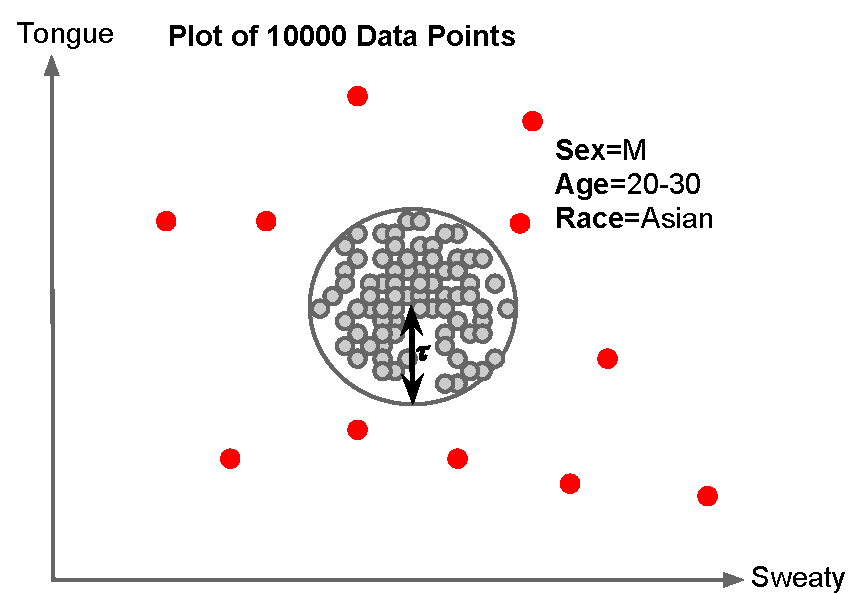
\includegraphics[width=0.9\columnwidth]{experiment/outlinerDetection-crop}
\caption{Outliner Detection}
\label{fig:outliner}
\end{figure}

\subsubsection{Model using $F_c$ and $F_s$}
$M$ is a model for fast cycle. 
We regard every parameter in $F_s$ as a $M_i^s$. $M_i^s$ is $1$ 
if the value is an abnormal value based on $F_p$ of that person; 
otherwise, $M_i^s$ is $0$. 

\begin{equation}
  M_i^s=\begin{cases}
    1, & \text{if $F_s$ is abnormal, given $F_p$}.\\
    0, & \text{otherwise}.
  \end{cases}
\end{equation}

$$M=max(M_c,M_1^s,M_2^s,M_3^s,M_4^s)$$

Parameters of $M_c$ are determined based on feeling and experience of people. 
Therefore, it is possible that error may occur. 
$M_i^s$ and abnormal boundaries of them are scientific measurements. 
Therefore, even $M_c$ is $0$, if any $M_i^c$ is $1$, we should still regard $M$ as $1$ (abnormal). 
\section{Slow Cycle: Social Network Model}\label{sec:slowCycle}

{\bf To Yingjie, could you please fill up this section?}
% \input{problemStat}
\section{Experiment}\label{sec:exp}


\subsection{Experiment Design}

\subsubsection{Fast Cycle}
In this experiment, we want to evaluate the effectiveness of our outliner detection model in Section~\ref{sec:outliner}. 
We want to show that:
\begin{enumerate}
 \item most people are healthy people and they would have similar $F_c$, and 
 \item most people can approximately determine their $F_c$. 
\end{enumerate}


Since we are unable to obtain real $F_c$ data, in this experiment, we will use similar data to evaluate the 
effectiveness of our proposed model. 
% We ask workers in Amazon Mechanical Turk to understand what are Tongue and sweaty 
We perform our experiment in Amazon Mechanical Turk. 
Given 5 pictures of 5 different faces, we ask 1000 workers to determine the size of nose, eyes, and mouth in every picture. 
For all 5 pictures, persons in the pictures have similar size of nose, eyes, and mouth. 
Worker can offer a score from 1 to 5, where 1 is the smallest size and 5 is the biggest size. 
Then, we put all data points together and build a model using method in Section~\ref{sec:outliner}. 
We want to show that it is possible to find a dense region in all data points, which implies 
most people would have similar sense while a small number of people are different from majority and people are able to 
offer approximate score for things that they understand. 


\subsubsection{Slow Cycle}
{\bf To Prof. Liang, could you please fill up this sub-section?}



% \input{relatedWork}

\bibliographystyle{abbrv}
\bibliography{review}  % sigproc.bib is the name of the Bibliography in this case
% You must have a proper ".bib" file
%  and remember to run:
% latex bibtex latex latex
% to resolve all references
%
% ACM needs 'a single self-contained file'!
%
%APPENDICES are optional
%\balancecolumns

% That's all folks!
\end{document}
